\documentclass[10pt]{extarticle}

% Lingua e matematica
\usepackage[english]{babel}
\usepackage{amsmath,amssymb,amsthm}

% Grafica e tabelle
\usepackage{graphicx}
\usepackage{subcaption}
\usepackage{float}
\usepackage{booktabs}
\usepackage{multirow}
\usepackage{siunitx}
\usepackage{wrapfig}
%\usepackage[section]{placeins}  % mantiene i float dentro la SECTION
%\let\Oldsubsection\subsection   % estendo il comportamento anche alle SUBSECTION
%\renewcommand{\subsection}{\FloatBarrier\Oldsubsection}
\usepackage{placeins}


% Codice (opzionale)
\usepackage{listings}
\usepackage{xcolor}
\definecolor{codegreen}{rgb}{0,0.6,0}
\definecolor{codegray}{rgb}{0.5,0.5,0.5}
\definecolor{codepurple}{rgb}{0.58,0,0.82}
\definecolor{backcolour}{rgb}{0.98,0.98,0.98}
\lstdefinestyle{mystyle}{
  backgroundcolor=\color{backcolour},
  commentstyle=\color{codegreen},
  keywordstyle=\color{magenta},
  numberstyle=\tiny\color{codegray},
  stringstyle=\color{codepurple},
  basicstyle=\ttfamily\footnotesize,
  breaklines=true, keepspaces=true, numbers=none, tabsize=2
}
\lstset{style=mystyle}

% Margini
\usepackage[margin=0.6in]{geometry}
\usepackage{ragged2e}
\usepackage{enumitem}
%\usepackage[utf8]{inputenc} % per caratteri UTF-8 nei .tex e nel .bib
\usepackage[backend=biber,style=ieee,sorting=none,maxbibnames=99]{biblatex}
\ExecuteBibliographyOptions{doi=true,url=true,isbn=false}
\addbibresource{references.bib}
\usepackage{csquotes}       % consigliato da biblatex (evita warning e parse strani)
\usepackage{pifont}
\newcommand{\good}[1]{\textcolor{teal!70!black}{\ding{51}~#1}}



% Bibliografia (biblatex + biber)
\usepackage[backend=biber,style=ieee]{biblatex}
\addbibresource{references.bib}

% TOC: includi anche \paragraph e numerali
\setcounter{secnumdepth}{2}
\setcounter{tocdepth}{2}

% Hyperref (sempre *dopo* gli altri pacchetti)
\usepackage[colorlinks=true,linkcolor=blue,citecolor=teal,urlcolor=magenta]{hyperref}


\begin{document}

% Custom header without a separate titlepage
\noindent
\begin{minipage}{0.3\textwidth}
    
\includegraphics[width=1.3\linewidth]{Figures/polito_logo_2021_blu.jpg}
\end{minipage}
\hfill
\begin{minipage}{0.68\textwidth}
    \raggedleft
    {\LARGE \textbf{Politecnico di Torino}}\\[0.2cm]
    {\large Master's Degree in Mathematical Engineering}\\[0.7cm]
    {\large \textbf{Material for Thesis}}\\[0.2cm]
    {\large d-- Data Pre-processing Pipeline \\ Comparison with An empirically driven data reduction
method on the human 450K methylation
array to remove tissue specific non-variable
CpGs
}
\\[0.7cm]
    \begin{tabular}{rl}
        Elisabetta Roviera & \texttt{s328422} \\
    \end{tabular}
\end{minipage}

\vspace{1cm}
\hrule
\vspace{0.5cm}

\tableofcontents

\vspace{0.5cm}
\hrule
\vspace{1cm}


% Main content begins here, on the same page
\justifying

\begin{abstract}
This document presents an extension of an empirically driven data reduction framework for DNA methylation data, adapting it to a breast cancer epigenomic context. Breast tissue is introduced as an additional reference in order to assess the robustness of non-variable CpG selection under increased biological heterogeneity.

The analysis evaluates cross-tissue overlap, selection stability, and baseline methylation and variability properties of the resulting CpG sets. The proposed framework defines the final structural step of the data pre-processing pipeline, yielding a stabilized CpG feature space for subsequent feature selection and downstream analyses.

The complete implementation is available at
\href{https://github.com/elisabettaroviera/THESIS/blob/main/01%20-%20Notebook/02%20-%20Data%20Pre-Processing/02-extention-of-edgar-s-study.ipynb}{\texttt{02-extention-of-edgar-s-study.ipynb}}.
\end{abstract}



\section{Empirically Driven Filtering of Non-Variable CpGs}

\paragraph{Motivation}
Epigenome-wide association studies (EWAS) based on Illumina HumanMethylation450K arrays typically investigate subtle DNA methylation changes, while simultaneously testing more than 450,000 CpG sites. In this setting, the multiple testing burden substantially limits statistical power, particularly when true effect sizes are small.

A key empirical observation is that a large fraction of CpG sites exhibit minimal variability within a given tissue. Such CpGs are structurally uninformative for tissue-specific analyses, yet they contribute to the dimensionality of the testing space and to the associated statistical penalty.

\paragraph{Filtering strategy}
An empirically driven filtering strategy addresses this issue by identifying CpG sites that are consistently non-variable within a tissue using independent reference datasets. Rather than defining variability solely within the dataset under analysis, reference-based non-variable CpG lists are derived from large collections of publicly available methylation data and subsequently applied as a biologically informed dimensionality reduction step.

\paragraph{Reference data and definition of non-variability}
Illumina 450K datasets from healthy blood, buccal epithelial cells, and placenta were used as reference tissues. Cancer samples were excluded in order to estimate baseline methylation stability. After standard quality control procedures, non-variable CpGs were defined as sites whose beta-value range between the 10th and 90th percentile was smaller than 5\%.

This criterion is designed to capture CpGs with minimal natural variability at the population level, independently of any phenotype or group comparison.

\paragraph{Resulting non-variable CpG sets}
Applying this definition yields large tissue-specific non-variable CpG sets, accounting for approximately 20--30\% of the array. These CpGs are enriched in CpG islands and promoter regions and are predominantly associated with extreme methylation states. The resulting lists were shown to be robust across preprocessing pipelines and normalization strategies.

\paragraph{Intended use}
The purpose of this filtering strategy is to reduce the dimensionality of methylation data prior to downstream analysis, thereby improving statistical power and robustness. The approach is intended as a general preprocessing step and is directly extensible to higher-density platforms.

\section{Extension to Breast Tissue and Cross-Tissue Stability}

The empirically driven filtering strategy described above is extended by incorporating breast tissue as an additional reference. The objective is to assess whether CpGs identified as non-variable in population-study tissues preserve this property when a cancer-relevant tissue is included, without modifying the original definition of non-variability.

Introducing breast tissue reframes non-variability as a robustness constraint rather than a purely tissue-specific property. Cross-tissue comparison reveals a shared subset of CpGs that remain non-variable across all considered tissues, alongside tissue-exclusive components. The persistence of a shared core despite the inclusion of a biologically heterogeneous tissue supports the interpretation of non-variability as a stable, context-independent property for a subset of CpGs.

At the same time, the presence of sizable tissue-specific components indicates that non-variability is not universal. The resulting shared subset is therefore more conservative than that obtained from healthy tissues alone, providing a stricter baseline suitable for cancer-oriented analyses.

This assessment motivates a structured refinement of the filtering strategy, articulated through the following steps:

\begin{itemize}[label=-]
\item \textbf{Step A}: evaluation of selection robustness under dataset perturbations.
\item \textbf{Step B}: analysis of the trade-off between stability and dimensionality reduction.
\item \textbf{Step C}: characterization of methylation distributions of selected CpGs.
\item \textbf{Step D}: assessment of baseline variability behavior across CpG subsets.
\end{itemize}

Together, these steps formalize the selection of a stabilized CpG feature space.


\begin{figure}
\centering
\begin{subfigure}[t]{0.48\textwidth}
  \centering
  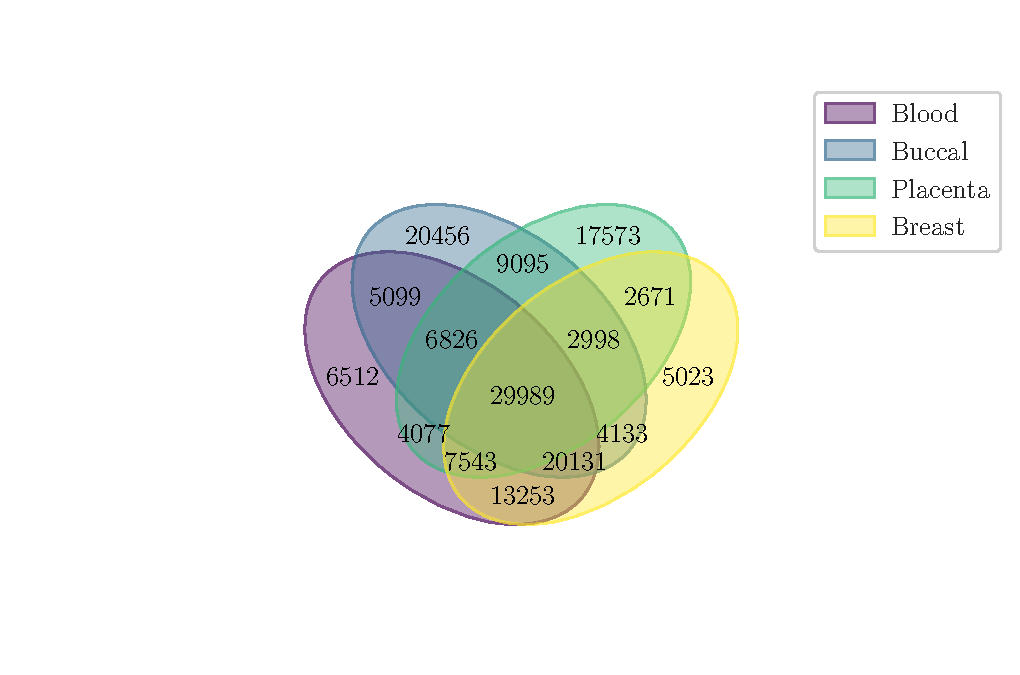
\includegraphics[width=\textwidth]{Figures/venn_4tissues_invariants.pdf}
  \caption{Overlap of tissue-specific non-variable CpGs across blood, buccal, placenta, and breast tissue.}
  \label{fig:venn_4tissues}
\end{subfigure}
\hfill
\begin{subfigure}[t]{0.48\textwidth}
  \centering
  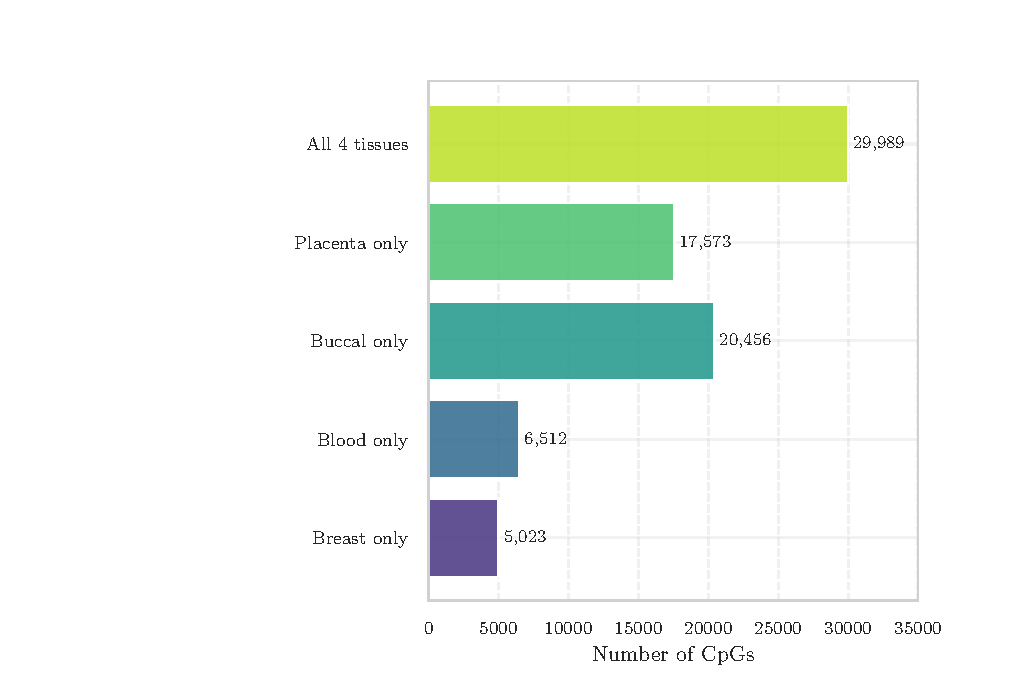
\includegraphics[width=\textwidth]{Figures/barplot_key_intersections_invariants.pdf}
  \caption{Key intersection sizes, highlighting tissue-exclusive components and the four-way shared core.}
  \label{fig:barplot_key_intersections}
\end{subfigure}

\caption{Global structure of non-variable CpGs across tissues, combining qualitative overlap (Venn diagram) and quantitative summary (bar plot).}
\label{fig:point0_global_structure}
\end{figure}


\subsection{Step A: Stability of non-variable CpG selection}

This step evaluates the robustness of the non-variable CpG selection procedure by assessing its sensitivity to dataset composition. To this end, a leave-one-dataset-out (LODO) strategy was adopted, whereby the non-variable CpG set is recomputed after excluding one dataset at a time, and compared against the reference set obtained using the full collection of datasets.

The resulting retention rates, reported in Figure~\ref{fig:stepA_lodo}, quantify the fraction of CpGs retained in each LODO configuration relative to the full-reference set. Across all held-out datasets, high retention values are observed, indicating that the selection of non-variable CpGs is not driven by any single dataset, but rather reflects a stable property of the underlying methylation variability structure.

This result is methodologically important, as it demonstrates that the identification of non-variable CpGs is robust to dataset perturbations and does not rely on specific cohort characteristics. In the context of extending the Edgar framework to a cancer-relevant tissue, such robustness is a necessary condition for interpreting non-variability as a genuine empirical property rather than an artifact of dataset composition.

\subsection{Step B: Trade-off between stability and dimensionality reduction}

While Step A establishes the robustness of the non-variable CpG selection under a fixed definition, Step B investigates how this robustness depends on the choice of the non-variability threshold. Specifically, this step explores the relationship between selection stability and the size of the resulting CpG list as the variability threshold is varied.

Figure~\ref{fig:stepB_stability_vs_size} summarizes this relationship by jointly reporting the mean Jaccard similarity across LODO folds and the corresponding mean number of non-variable CpGs as a function of the threshold. As expected, increasing the threshold leads to larger CpG sets, accompanied by higher stability across LODO configurations. Conversely, stricter thresholds yield smaller lists that are less stable due to increased sensitivity to dataset-specific variability.

The highlighted configuration corresponding to the threshold originally proposed by Edgar et al.~represents a balance between robustness and dimensionality reduction. At this operating point, the selected CpG set achieves substantial stability while maintaining a meaningful reduction in feature space. This observation provides an empirical justification for retaining the original threshold in the extended framework and supports its use as a principled compromise between reproducibility and filtering strength when breast tissue is included in the analysis.

\begin{figure}
\centering
\begin{subfigure}[t]{0.48\textwidth}
  \centering
  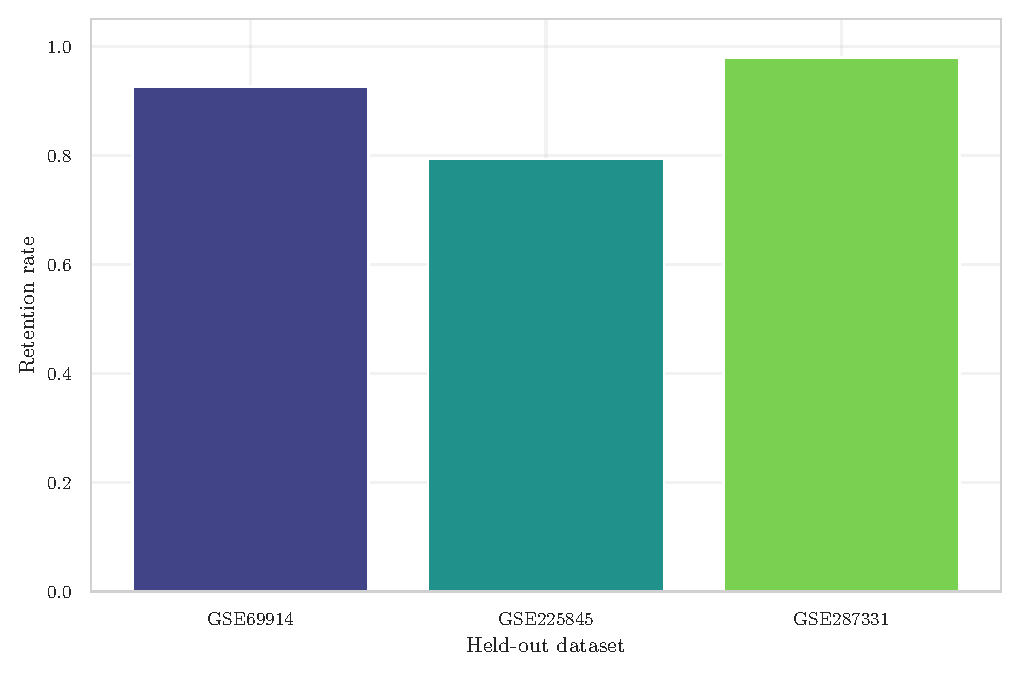
\includegraphics[width=\textwidth]{Figures/stepA_lodo_stability.pdf}
  \caption{Step A: stability of non-variable CpG selection under a leave-one-dataset-out (LODO) strategy.}
  \label{fig:stepA_lodo}
\end{subfigure}
\hfill
\begin{subfigure}[t]{0.48\textwidth}
  \centering
  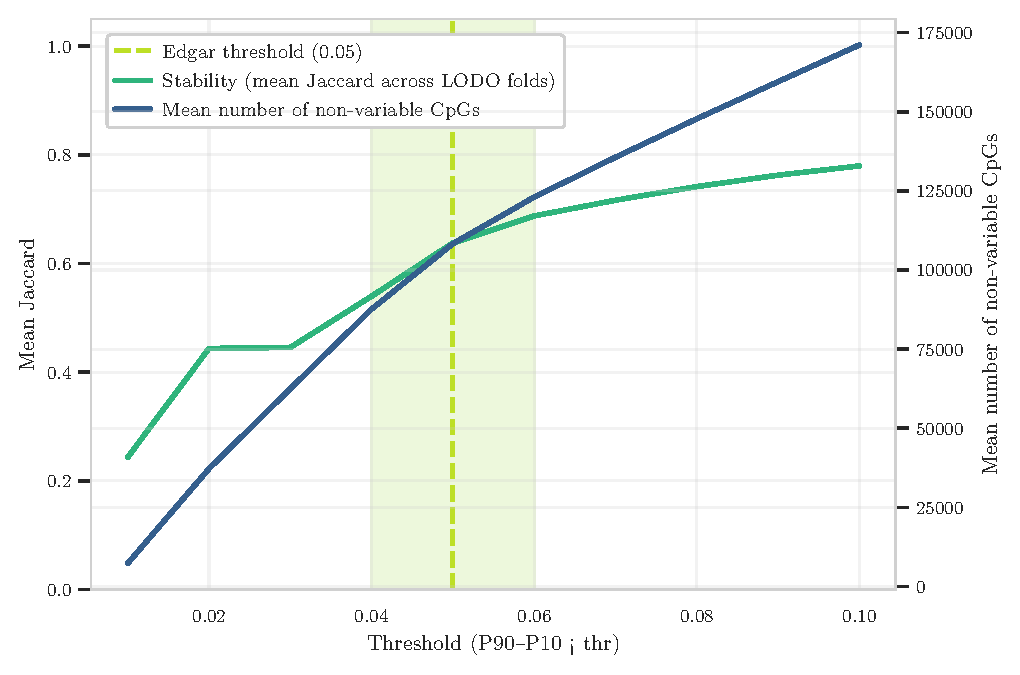
\includegraphics[width=\textwidth]{Figures/stepB_stability_vs_list_size_highlighted.pdf}
  \caption{Step B: relationship between stability and list size, with the selected configuration highlighted.}
  \label{fig:stepB_stability_vs_size}
\end{subfigure}

\caption{Step A--B: assessment of robustness and trade-off between stability and dimensionality of non-variable CpG sets.}
\label{fig:stepAB}
\end{figure}


\subsection{Step C: Methylation distribution of selected non-variable CpGs}

This step characterizes the methylation profiles of the selected non-variable CpGs by comparing their beta-value distribution to that of a background set of CpGs. The analysis focuses on beta values computed on normal samples, pooled across datasets, in order to assess whether the selected CpGs exhibit distinctive methylation patterns relative to the genomic background.

The distribution shown in Figure~\ref{fig:stepC_beta_distribution} reveals that non-variable CpGs in breast tissue are strongly concentrated at extreme beta values, close to 0 or 1, whereas the background CpGs display a much broader distribution spanning the full beta-value range. This separation indicates that the lack of variability observed for the selected CpGs is associated with stable hypo- or hypermethylated states, rather than intermediate methylation levels.

This observation is consistent with the original findings reported by Edgar et al.~\cite{Edgar2017}, who noted that non-variable CpGs tend to localize at extreme methylation states. Importantly, the same pattern is preserved when breast tissue is included, providing additional support for the interpretation of non-variability as a genuine empirical property of the methylation landscape rather than an artifact of tissue composition or disease-related heterogeneity.

\subsection{Step D: Baseline variability behavior across CpG subsets}

While Step C focuses on marginal methylation levels, Step D evaluates the behavior of the selected CpG sets with respect to baseline within-normal variability. To this end, the empirical cumulative distribution function (ECDF) of the variability measure $rr = P90 - P10$ was computed for multiple CpG subsets, including the four-way shared non-variable set, the breast-specific non-variable set, the breast-only non-variable set, and a random background set.

The ECDFs reported in Figure~\ref{fig:stepD_rr_ecdf} show a clear separation between the non-variable CpG subsets and the background. The majority of CpGs in the shared and breast-specific non-variable sets exhibit very low $rr$ values, with distributions concentrated well below the threshold originally proposed by Edgar et al.~ This contrasts sharply with the background distribution, which spans a substantially wider range of variability values.

This result provides a quantitative validation of the filtering strategy, demonstrating that the selected CpG sets are not only defined by construction as non-variable, but also empirically exhibit a distinct baseline variability profile. The consistency of this behavior across different non-variable subsets further supports the robustness of the extended framework and justifies the use of the selected CpG sets as stable baselines for downstream analyses in breast cancer epigenomic studies.

\begin{figure}
\centering
\begin{subfigure}[t]{0.48\textwidth}
  \centering
  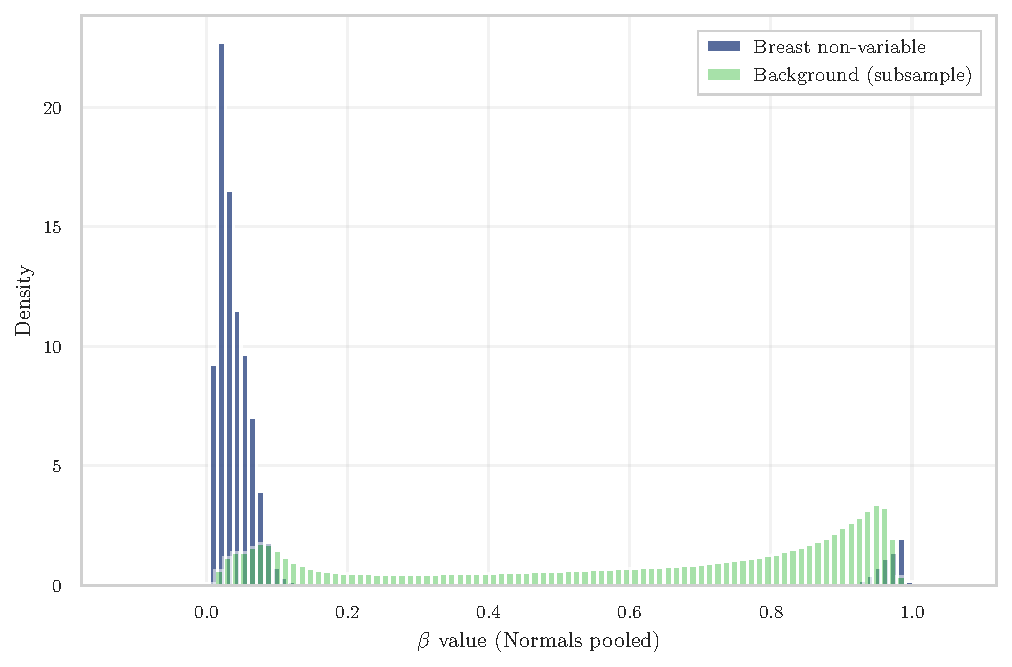
\includegraphics[width=\textwidth]{Figures/stepC_beta_distribution_nv_vs_background.pdf}
  \caption{Step C: distribution of beta values for non-variable CpGs compared to the genomic background.}
  \label{fig:stepC_beta_distribution}
\end{subfigure}
\hfill
\begin{subfigure}[t]{0.48\textwidth}
  \centering
  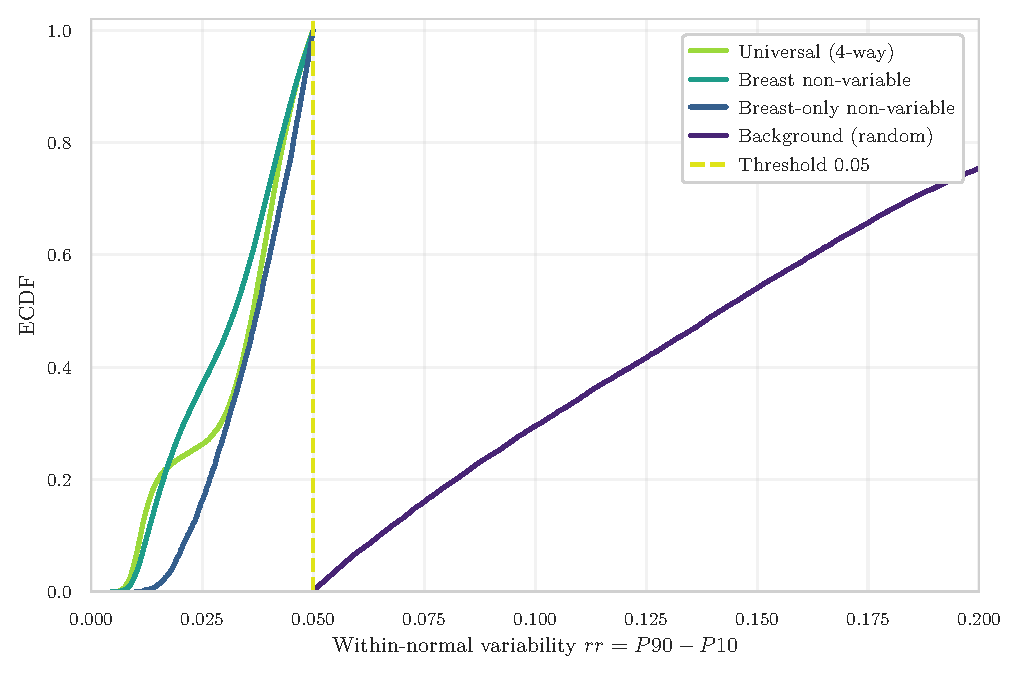
\includegraphics[width=\textwidth]{Figures/stepD_baseline_rr_ecdf.pdf}
  \caption{Step D: empirical cumulative distribution of baseline relative risk across CpG subsets.}
  \label{fig:stepD_rr_ecdf}
\end{subfigure}

\caption{Step C--D: characterization of the selected non-variable CpG set in terms of methylation distribution and baseline risk behavior.}
\label{fig:stepCD}
\end{figure}


\subsection{Positioning within the preprocessing pipeline}

This extended analysis constitutes the final step of the data pre-processing pipeline. By selecting CpG sites that are non-variable across multiple tissues, including a cancer-relevant tissue, it defines a conservative and empirically justified feature space.

All subsequent operations, including feature selection, differential methylation analysis, and predictive modeling, are performed on this reduced and stabilized CpG set. This separation ensures that downstream analyses operate on a feature space that has already been purged of structurally uninformative CpGs, improving robustness, interpretability, and computational efficiency.


\printbibliography
\end{document}
